\chapter{Конструкторский раздел}

    В данном разделе будут рассмотрены требования к программному обеспечению, а также схемы алгоритмов, выбранных для решения поставленной задачи. Так же, будут описаны пользовательские структуры данных и приведена структура реализуемого программного обеспечения.
    
    \section{Разработка алгоритмов}
    
        \subsection{Основные физические соотношения для дисперсии}
    
            Дисперсия света обусловлена зависимостью показателей преломления света от длины волны. Закон Снеллиуса (также Снелля или Снелла) описывает преломление света на границе двух прозрачных сред.
        
            Угол падения света на поверхность связан с углом преломления соотношением \eqref{eq:dis}:
        
            \begin{equation}
               n_{1} sin(\theta_{1}) = n_{2} sin(\theta_{2}) \label{eq:dis}
            \end{equation}
            
            где $n_{1}$ — показатель преломления среды, из которой свет падает на границу раздела;
            
            $\theta_{1}$ — угол падения света — угол между падающим на поверхность лучом и нормалью к поверхности;
            
            $n_{2}$ — показатель преломления среды, в которую свет попадает, пройдя границу раздела;
            
            $\theta_{2}$ — угол преломления света — угол между прошедшим через поверхность лучом и нормалью к поверхности.
            
    
            Формула Зельмейера \eqref{eq:zel} — это эмпирическая формула описывающая зависимость между показателем преломления и длиной волны для конкретной прозрачной среды. Уравнение используется для определения дисперсии света в этой среде. 
            
            \begin{equation}
                n^2(\lambda) = 1 + \sum_{i}^{} \frac{B_i \lambda^2}{\lambda^2 - C_i}  \label{eq:zel}
            \end{equation}
            
            где \( n \) - показатель преломления;
            
            \( \lambda \) - длина волны;
            
            \( B_i, C_i \) - экспериментально определяемые коэффициенты Селлмейера.
    
        \subsection{Пересечение луча и сферы}
        
            Уравнение луча представлено ниже:

            \begin{equation}
            	P = O + t\overrightarrow{D}, t \geq 0,
            	\label{eq:ref5}
            \end{equation}
            где \( P \) -- точка лежащая на луче, \( O \) -- начало луча, $\overrightarrow{D}$ -- направление луча, \( t \) -- произвольное положительное действительное число.
            
            Сфера — это множество точек $P$, лежащих на постоянном расстоянии $r$ от фиксированной точки $C$. Тогда можно записать уравнение, удовлетворяющее этому условию:
            
            \begin{equation}
            	distance(P,C) = r
            	\label{eq:ref6}
            \end{equation}
            
            Запишем расстояние (\ref{eq:ref6}) между P и C как длину вектора из P в C.
            
            \begin{equation}
            	|P-C|=r
            \end{equation}
            
            Заменим на скалярное произведение вектора на себя:
            
            \begin{equation}
            	\sqrt{\langle P - C\rangle, \langle P - C\rangle} = r
            \end{equation}
            
            Избавимся от корня:
            
            \begin{equation}
            	\langle P - C\rangle, \langle P - C\rangle = r^2
            	\label{eq:ref7}
            \end{equation}
            
            В итоге есть два уравнения - уравнение луча и сферы. Найдем пересечение луча со сферой. Для этого подставим (\ref{eq:ref5}) в (\ref{eq:ref7})
            
            \begin{equation}
            	\langle O + t\overrightarrow{D} - C \rangle, \langle O + t\overrightarrow{D} - C\rangle = r^2
            \end{equation}
            
            Разложим скалярное произведение и преобразуем его. В результате получим:
            
            \begin{equation}
            	t^2 \langle \overrightarrow{D}, \overrightarrow{D} \rangle + 2t \langle \overrightarrow{OC}, \overrightarrow{D} \rangle + \langle \overrightarrow{OC}, \overrightarrow{OC} \rangle -r^2 = 0
            	\label{eq:ref8}
            \end{equation}
            
            Представленное квадратное уравнение (\ref{eq:ref8}) имеет несколько возможных случаев решения. Если у уравнения одно решение, то луч касается сферы. Два решения -- луч пересекает сферу. Нет решений -- луч не пересекается со сферой.

        \subsection{Описание алгоритма обратной трассировки}
        
            Суть алгоритма состоит в следующем: Из некоторой точки пространства, называемой виртуальным глазом, или камерой, через каждый пиксель изображения испускается луч и находится точка пересечения с объектом сцены. При обнаружении точки пересечения, формируется отраженный луч и испускается. Данный алгоритм повторяется рекурсивно, пока не достигнем максимальной установленной глубины рекурсии. Полученные цвета перемножаются.

            На рисунке \ref{fig:ray_tracing} представлена схема синтеза изображения с применением данного алгоритма.

            \begin{figure}
                \centering
                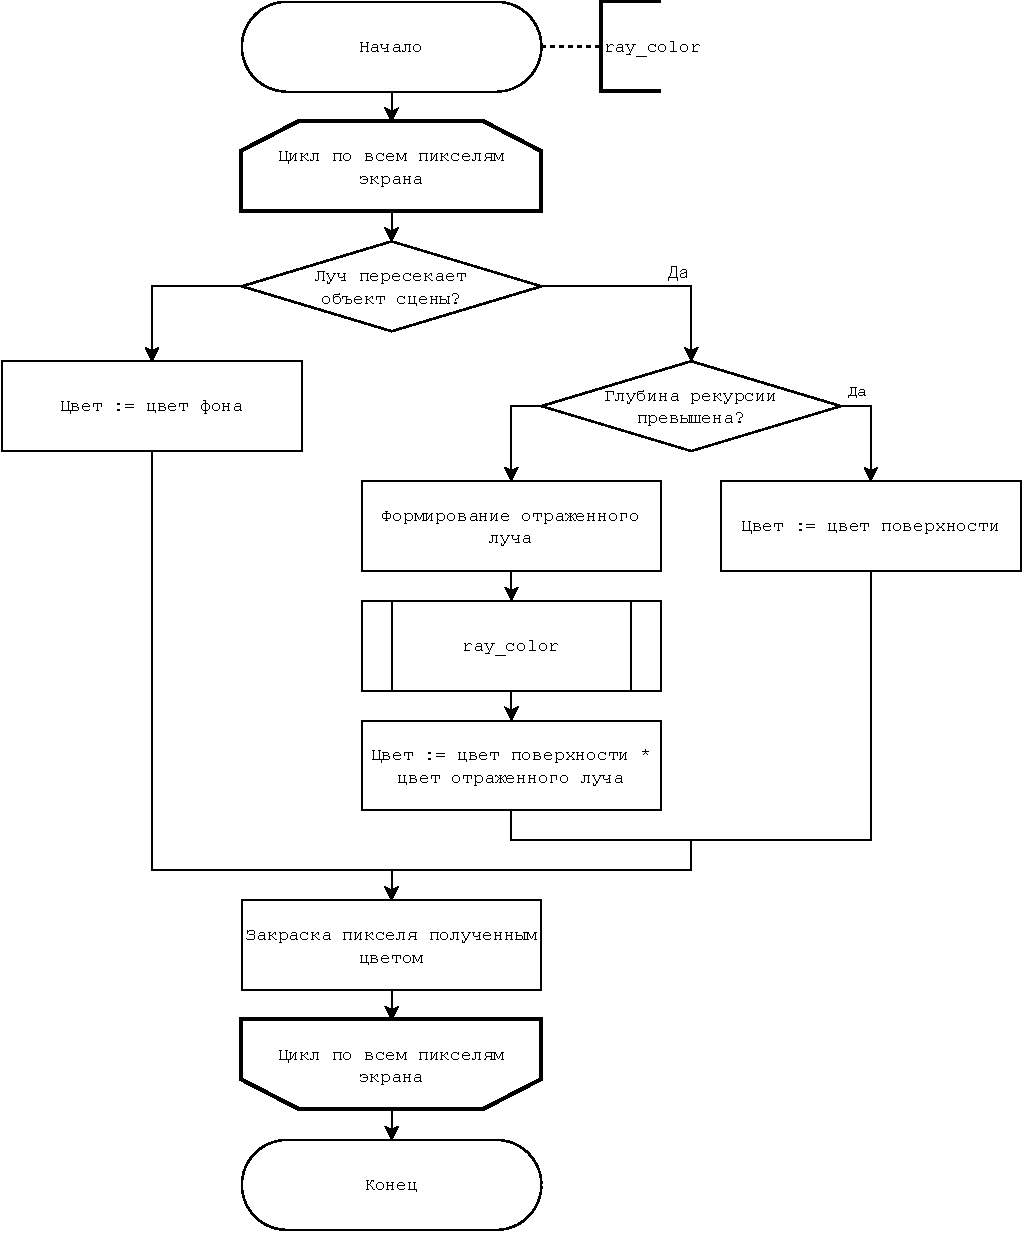
\includegraphics[width=\textwidth,height=25cm,keepaspectratio]{inc/img/ray_tracing.pdf}
                \caption{Схема алгоритма синтеза изображения с применением алгоритма обратной трассировки лучей} \label{fig:ray_tracing}
            \end{figure}

    \section{Описание используемых типов и структур данных}

        В данной работе используются следующие типы и структуры данных:
        
        \begin{itemize}
            \item источник света – задается расположением, направленностью и интенсивностью света;
            \item математические абстракции:
            \begin{itemize}
                \item точка -- хранит координаты x, y, z
                \item вектор -- хранит направление по x, y, z
            \end{itemize}
            \item цвет -- хранит три составляющие RGB модели цвета
        \end{itemize}

\clearpage

    \section{Описание структуры программного обеспечения}
    
            На рисунке \ref{fig:uml} представлена диаграмма классов реализуемого программного обеспечения. Объект класса \texttt{draw\_manager} генерирует изображение класса \texttt{image} для заданного положения камеры. Сцена состоит из объектов, удовлетворяющих интерфейсу \texttt{hittable}, который наследуют классы \texttt{sphere} и \texttt{hittable\_list}. Класс \texttt{hittable\_list} реализует паттер композит. Класс \texttt{sphere} агрегирует класс \texttt{material}, который в свою очередь алгегирует класс \texttt{texture}. Реализованы 4 типа материалов: матовый (\texttt{lambertian}), металлический (\texttt{metal}), прозрачный (\texttt{dieletric}), излучающий свет (\texttt{diffuse\_light}). И реализованы 2 типа текстур материалов: монотонный (\texttt{solid\_color}), клетчатый (\texttt{checker\_texture}).
        
        \begin{figure}
            \centering
            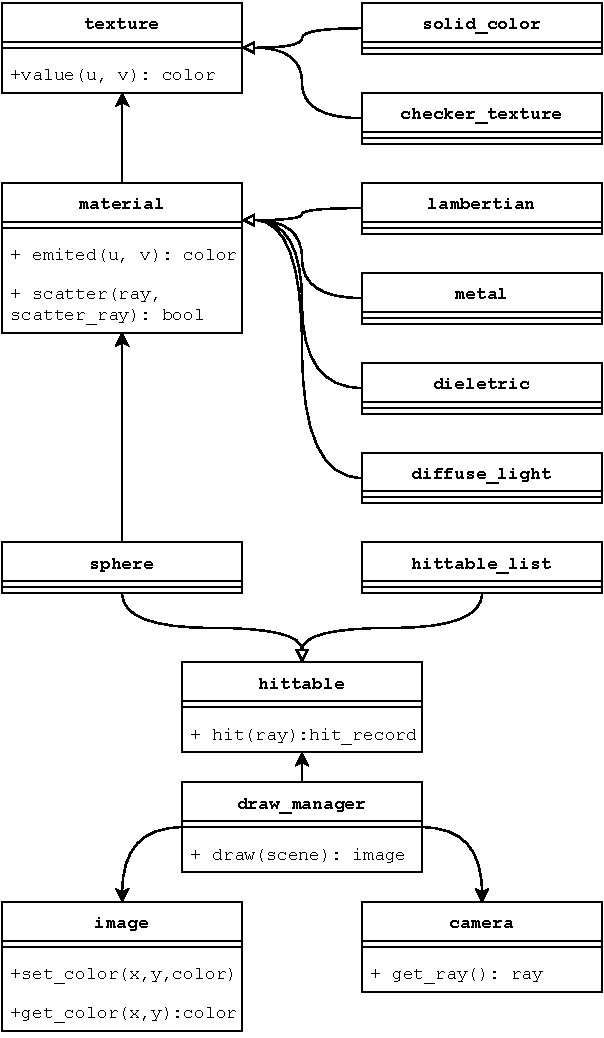
\includegraphics[width=\textwidth,height=25cm,keepaspectratio]{inc/img/uml.pdf}
            \caption{UML диаграмма разрабатываемого программного обеспечения}
            \label{fig:uml}
        \end{figure}

\clearpage

    \section{Вывод}

        В данном разделе были приведены основные физические соотношения для дисперсии, приведена схема алгоритма обратной трассировки лучей, описаны используемые структуры данных, приведена UML диаграмма разрабатываемого приложения.